This section presents simulation results that show how the  the planned impulses and the pattern of retraction force, 
obtained running  the optimization of Section \ref{sec:motionP}, are able to bring the robot to a desired target. 
The OCP solver used is PINS~\cite{pins:1,pins:2,pins:3}, which uses the indirect approach based on the Pontryagin Maximum Principle.

% 1st experiment: validation of optimization with 2 models, with obstacle
In a first experiment, we run the optimization to perform  a 12 $m$ jump starting from an initial 
position $p_0 = \mat{0.024& 0& -8}^T$ up to a target at $p_f = \mat{3 & 3 &-20}^T$ $[m]$. As additional constraint,
during the jump, the robot has to avoid a rock pillar (see the accompanying 
video\footnote{ \href{https://www.dropbox.com/s/b0fuyiewyp3jkg7/icra23climb.mp4}
{https://www.dropbox.com/s/b0fuyiewyp3jkg7/icra23climb.mp4} }) that is laying  the wall, that we model as a 20 $m$ high cone with a base of radius 2.5 $m$.
We validate the result of the optimization in the case of the simplified model (in a Matlab environment)
and for the full 3D model. In this case we built a Gazebo simulator based on the URDF  description \cite{urdf} of the robot.
The physical parameters of the robot and of the environment together with the 
optimization settings, are reported in Table \ref{tab:params}:
%
\begin{table}[H]
	\centering
	\caption{ Simulations parameters}
		\begin{tabular}{l c c  } \hline\hline
			\textbf{Name} \quad                  & \textbf{Symbol}                     & \textbf{Value}  \\ \hline
					Robot mass                   & m  & 5                 \\ 
					Max. impulse  [N]       	 & $F_{u}^{\text{max}}$				& 1000   \\
					Max. retraction force [N]    & $F_r^{\text{max}} $			& 200    \\
					Friction coeff.				 & $ \mu $ 					        & 0.8   \\
					Thrust impulse duration	[s]  & 	$T_{th}$  				& 0.025\\
					Discretization steps         & N 						& 20\\					        
			\hline\hline 					    					    					    
		\end{tabular}
		\label{tab:params}
\end{table}
%
For the Matlab simulation we simply integrate equation \eqref{eq:nonlinearDyn} 
with a ode45 Runge Kutta variable-step integration scheme.
For the Gazebo simulation, we assume to apply the push impulse as a force $F_c$ at the contact point.
Therefore we employ the leg dynamics to define the mapping between the contact force $F_c$ and the torques $\tau_{\text{leg}}$ at the leg joints:
%
\begin{equation}
\tau_{\text{leg}}^d= \mat{\tau_{HP} \\ \tau_{HR} \\ f_{K}} =  h_{\text{leg}} -J_{\text{leg}}^T \underbrace{\left(R_e^\mathcal{W}  \mat{F_{u,n} \\ F_{u,t} \\ 0} \right) 	}_{F_c}
\end{equation}
%
Where $J_{\text{leg}} \in \Rnum^{3 \times 3}$ is the sub-matrix of the Jacobian $J$ relative to the leg jonts, $R_b^\mathcal{W}$ is the rotation matrix 
that represents the orientation of the base link w.r.t. the inertial frame $\mathcal{W}$ (different from $R_e^\mathcal{W}$) and $h_{\text{leg}} \in \Rnum ^3$
represents the bias terms (Centripetal, Coriolis, gravity). Note that  we do
no generate any impulse along the rope direction (base link $Z$ direction) in 
order to avoid to accidentally create  any slack on the rope.
Additionally, to avoid complexity, we implement  virtual dampers to keep the passive joints at the 
base in a fixed position in order to avoid the angular motions, since the optimization is performed 
considering the simplified model that neglects the angular dynamics. 

We set the initial configuration to $q_0= \mat{ \atandue(r_{\text{leg}}, l_0) & 0 &0  & l_0 & 0 &  0 & 0  & -1.57  & 0 & 0}^T$ 
where $l_0$ is the initial rope length and $r_{leg}=0.38$ $m$ is the leg length at the startup configuration. 
At $q_0$  the foot is meant to touch the wall in $p_0$, the starting point of the optimized trajectory.
A state machine coordinates the 3 phases of the jump: leg orientation, thrusting and flying. 
In the leg orientation phase,  the hip roll joint set-point $q_{HR}^d$ is commanded
to have the leg aligned with the impulse direction, $q_{HR}^d = \atandue(\text{max}(F_{u,t}), \text{max}(F_{u,n}))$. 
Note that the hip-pitch joint set-point is $q_{0, HP}^d = -1.57$ in order to 
have the leg lying on the X-Y plane of the base frame. A low level PD controller 
runs in parallel with the  feed-forward actions $\tau_{\text{leg}}^d$ to drive the joints.  
During the \textit{thrusting} phase the force $F$ is generated at the contact 
applying $\tau_{\text{leg}}$ for a time $T_{th} = 0.025 s$, while the PD gains are 
switched off to avoid conflicts. Then  it follows  the 
flying phase, where   the rope winding joint is actuated with the optimized force pattern $\tau_R = F_r(t)$ for the whole jump duration $T_f$.

% computation time and number of nodes
The computation time for the optimization and the integration error at the target $\Vert e_f \Vert$  are linearly  
linked to the number of discretization points $N$. In Table~\ref{tab:solve_time} we report 
also the integration error normalized for the jump length $\Vert e_f \Vert / (l_f-l_0)$ 
for  different numbers of discretization points. 
%%%
\begin{table}[h!]
\centering
	\caption{ Results of the numerical OCP for different discretisations}
	\label{tab:solve_time}
	\begin{tabular}{c c c c  } \hline\hline
		\textbf{N} \quad & \textbf{Comp. time [s]}           & \textbf{$\Vert e_f \Vert$ [m]} &  \textbf{$\Vert e_f \Vert / (l_f-l_0)$ [\%]} \\ \hline
			250    &   0.850          &  0.0937 & 0.76 \\
			500    &   1.472          &  0.0525 & 0.42 \\
			1000   &   2.648          &  0.0238 & 0.19 \\
			2000   &   5.063          &  0.0180 & 0.14 \\
		\hline\hline 					    
	\end{tabular}	
\end{table}


In Fig. \ref{fig:validation}  we report the results of the validation. 
The discrepancy in the target position is mainly due to drift in the integration in the case of Matlab and to the approximation
of the simplified model with respect to the real one in the  case of Gazebo simulation. 
These results in errors in the generation of the impulse that require 
However in both cases the norm of the error is always below XX which shows the simplified model is a good approximation for the real system.
The friction constraints are also fulfilled therefore initially the robot has to lift-off 
with an angle limited by the friction cone. However, since the target location is out of the cone (with vertex at the initial position)
the optimizer should "steer" the trajectory and therefore it dictates  an \textit{initial} 
retraction of the rope to vary the time constant of the "pendulum", 
then the rope passively unwinds  under the action of gravity.
An interesting outcome of this analysis is that despite the system is fully controllable (locally) 
the reachable targets, when jumping  from the anchor line, are limited to the area inside the cone, 
therefore to move tangentially \textit{away} from the anchor line  
only small jumps can be performed. Conversely, the jumps have no limit when jumping toward the anchor line, 
because the gravity component (always pointing toward the anchor line) can be exploited. 

\begin{figure}[H]
	\includegraphics[width=\columnwidth]{matlab/validation.pdf}
	\caption{\small Simulation. Validation of the optimization results. The red line is the  \gls{com} trajectory computed by the optimization. 
		The blue and black lines are the simulated trajectory with Matlab and Gazebo, respectively. 
		The bottom plot is the rope retraction force $F_r(t)$.}
	\label{fig:validation}
\end{figure}

 
% multiple targets
Additionally, we ran the optimization for  several targets on the wall (see Fig. \ref{fig:targets}) and we 
validated the output of the optimization both  with the simplified and the detailed model. 
Each optimization provided the initial impulses ($Fun$, $Fut$), the pattern of the winding force $F_r$ and the jump duration $T_f$.
We terminate each simulation after the jump time $T_f$ is elapsed and computed the norm of the error from the target. 
We selected the target points inside the shaded red area that represents the friction boundaries in the tangential direction.

The results are the reported in Table \ref{tab:sim_different_targets}. 
Note that, as expected, the error increases with the distance of the target.

\begin{figure}
	\includegraphics[width=\columnwidth]{matlab/targets.pdf}
	\caption{\small Simulation. The red line is  the trajectory of the \gls{com} computed by the optimization, 
		the blue and black line is the simulated trajectory with Matlab and Gazebo, respectively.}
	\label{fig:targets}
\end{figure}

\begin{table}[h!]
	\centering
	\caption{ Matlab simulations results}
	%	\renewcommand{\arraystretch}{1.1}
	\resizebox{\columnwidth}{!}{
		\begin{tabular}{c c c c c c  c } \hline\hline
			\textbf{Test} \quad & \textbf{$p_f$ [m]}           & \textbf{$T_f$ [s]} &  \textbf{$F_{un}$ [N]} & \textbf{$F_{ut}$ [N]} 
			\footnote{The value of these forces are related to the selected impulse duration $T_{th}$  [s], they can be strongly reduced by taking longer durations (i.e. in accordance to the actuator  response time).} 
			&\textbf{ $E_{k,f}$ [J]}\\ \hline % & \textbf{$\Vert e \Vert$ [m]}
			1   & $\mat{4.0  & 5.0 &  -8}^T $&      2.16      &         780             &      624           &    408    \\
			2     & $\mat{1.0& 1.0& -8}^T$ &        1.57        &         241             &      192           &    6.5               \\
			3  & $\mat{4.0  & 1.0 &  -8}^T $&      1.2         &       746                  &   200              & 11.8               \\
			4   &$ \mat{2.0  & 2.0 &  -6}^T $&      1.54       &        504              &     403         &      22    &                 \\
			5   &$ \mat{1.0  & 0.0 &  -6}^T $&      0.95     &           180           &      -1.65           &    2.40             \\
			\hline\hline 					    					    					    
		\end{tabular}}
		\label{tab:sim_different_targets}
 \end{table}
 
We  noticed that, due to the physics of the system, in order to reach lateral targets  the optimization is trying to rewind the  rope 
to steer the trajectory that would be otherwise  be limited by a plane linked to the value  the friction coefficient. Therefore, we performed a reachability analysis 
to plot the region (see Fig.  \ref{fig:reachable_region})  of reachable targets for a friction coefficient of $\mu =1.3$, performing a number of optimizations. 
We selected this quite large value for $\mu$ because it is reasonable to assume that  the 
robot will  exploit the asperities present on a rocky wall  perform the push, which provide a reasonable amount of tangential impulse. 

\begin{figure}[H]
%	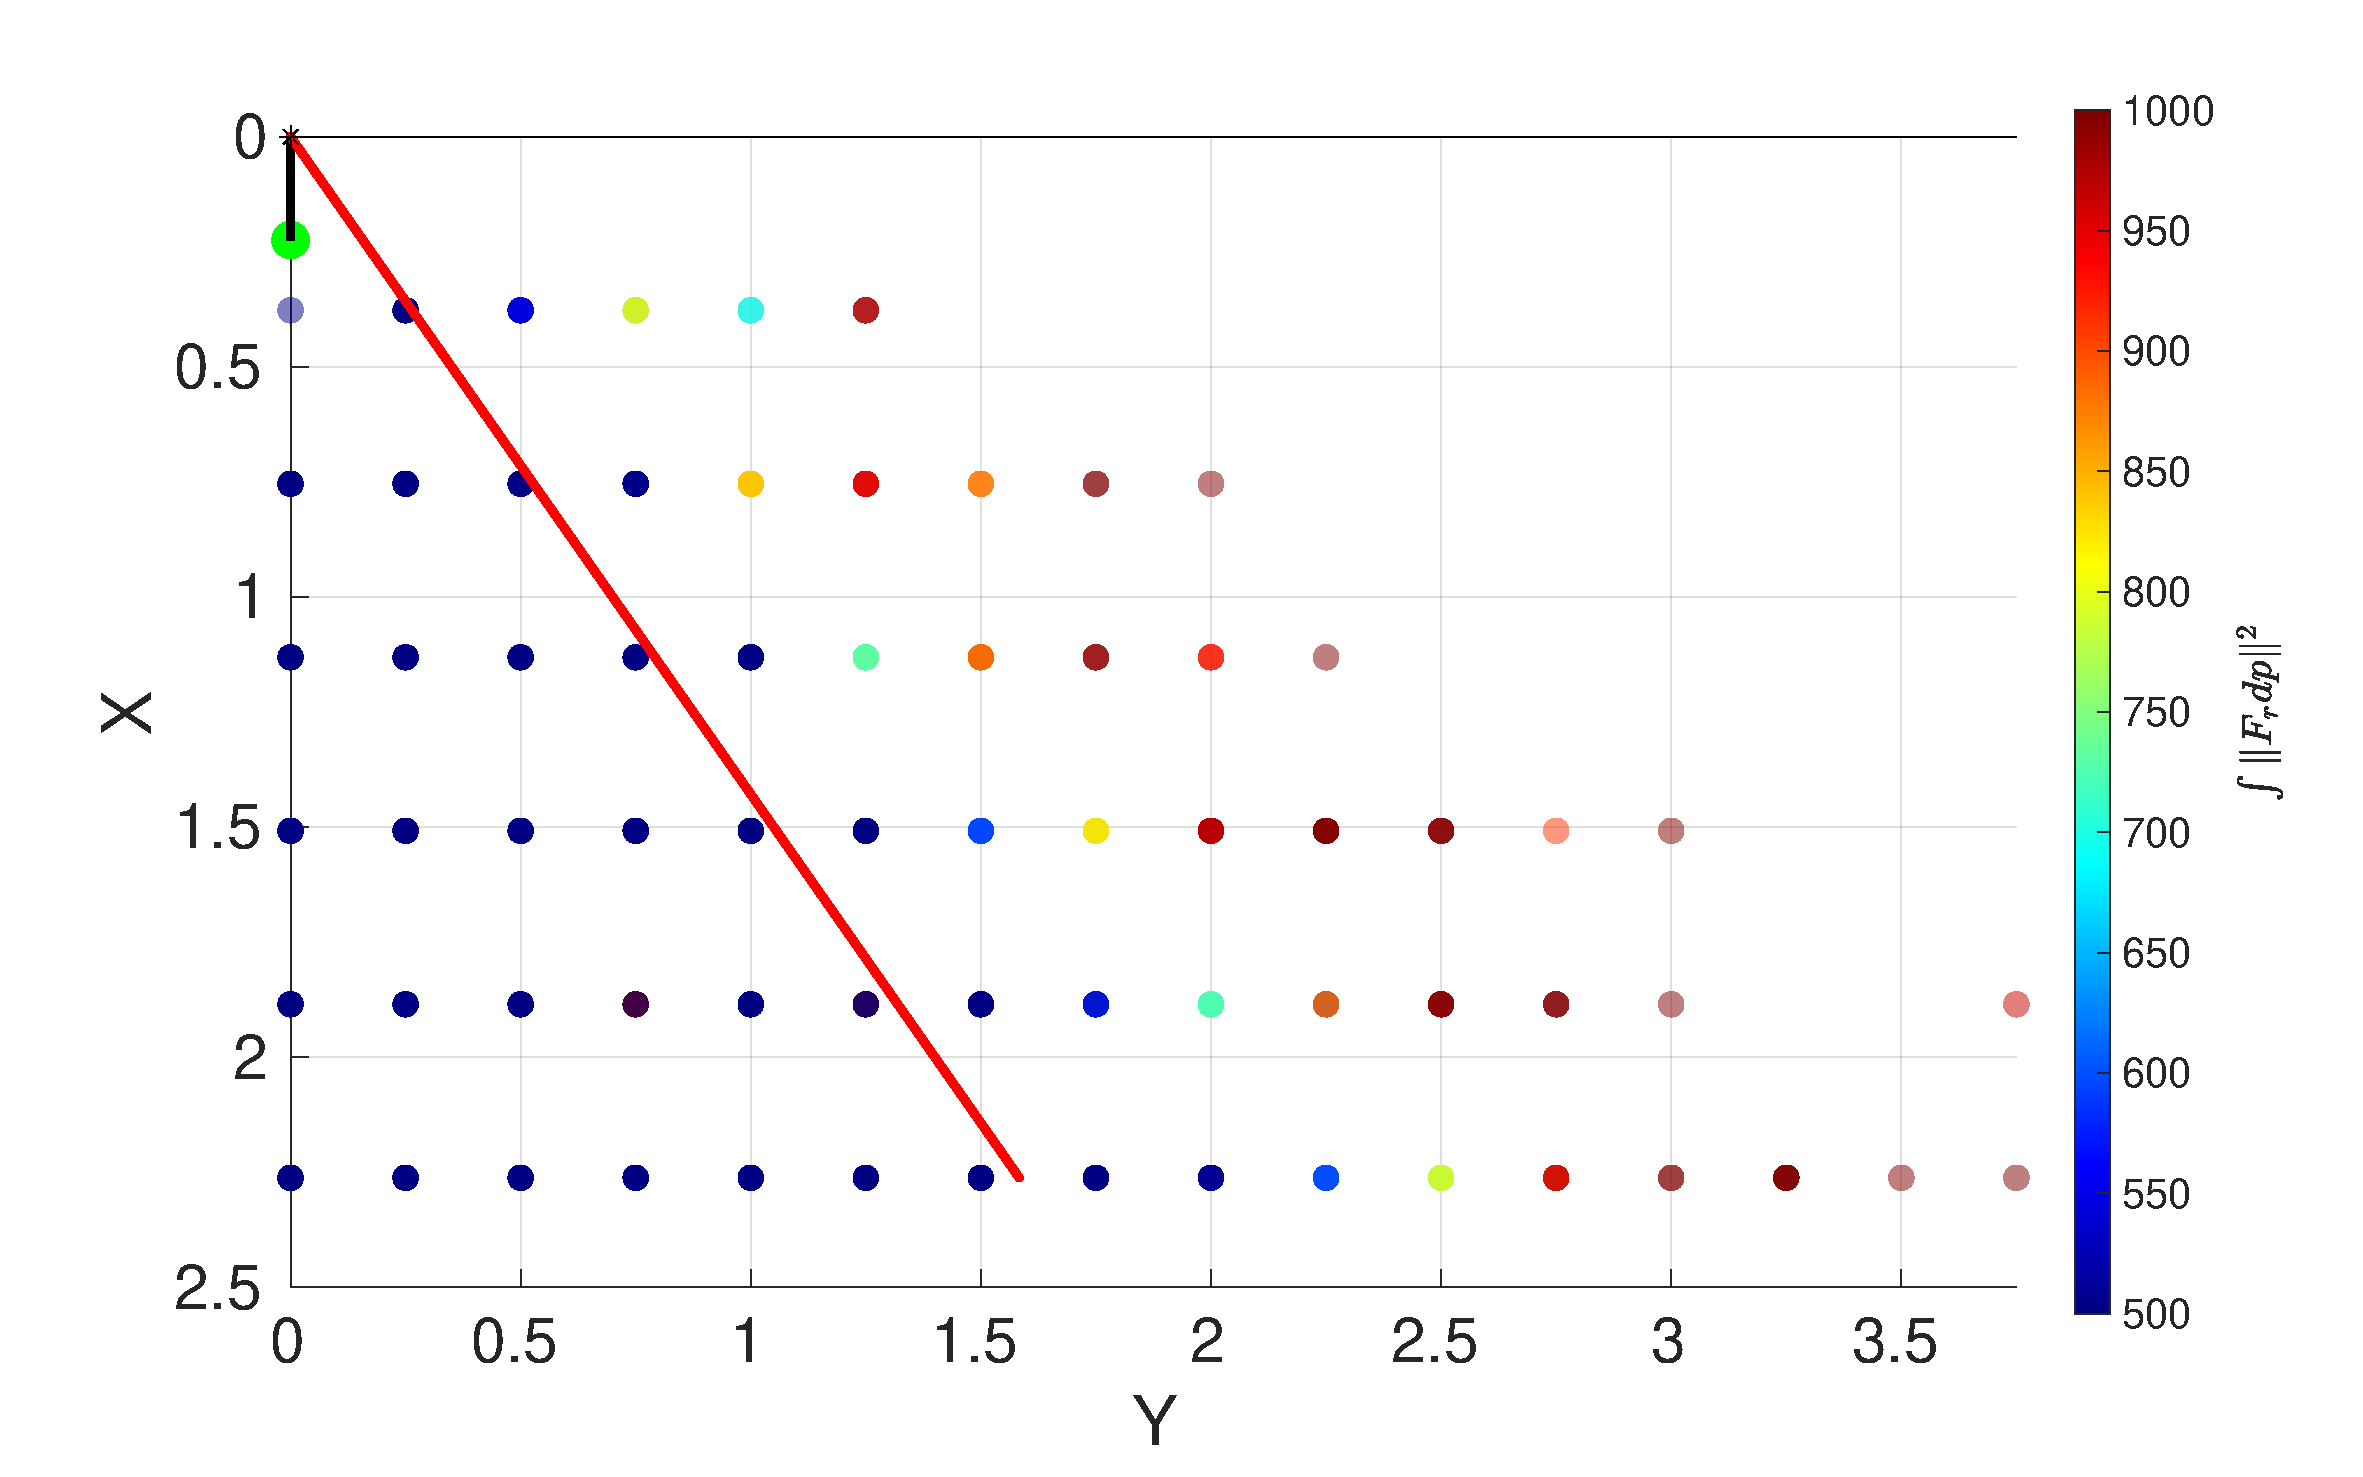
\includegraphics[width=\columnwidth]{matlab/reachable.pdf}
	\caption{\small Simulation. Plot of the region of reachable targets for a friction coefficient $\mu$.}
	\label{fig:reachable_region}
\end{figure}
